\documentclass{article}

% imports
\usepackage{xcolor}     % colorize text
\usepackage{graphicx}   % images
\usepackage{hyperref}   % hyperlinks
\usepackage{float}      % better image positioning
\usepackage{gensymb}    % include degree in math mode

% overrides & setup
\usepackage[nottoc,numbib]{tocbibind}               % include refs in toc
\usepackage[figurename=Abbildung]{caption}          % rename figures
\renewcommand{\refname}{Quellen}                    % rename references
\renewcommand{\contentsname}{Inhaltsverzeichnis}    % rename toc
\graphicspath{{./images/}}
\hypersetup{
    colorlinks=true,
    linkcolor=black,
    citecolor=black,
    filecolor=black,
    urlcolor=black,
}

\begin{document}
    \begin{titlepage}
    \begin{center}
        \Huge
        \textbf{Solarzellen}

        \vspace{0.5cm}

        \LARGE
        Funktion und Stand der Technik bei Stand-Alone-Anlagen

        \vspace{1.5cm}

        \href{mailto:erik.buennig@fh-erfurt.de}{
            \color{black}{
                \textbf{Erik Bünnig}
            }
        }\\
        18.2.2021

        \vfill

        \Large
        Projektarbeit zur alternativen Prüfungsleistung im Kurs Elektrotechnik

        \vspace{1.5cm}

        \href{https://www.fh-erfurt.de/fhe/}{
            
\includegraphics[scale=0.5]{fhe_logo}
        }
    \end{center}
\end{titlepage}

    \tableofcontents
    \thispagestyle{empty}
    \newpage

    \pagenumbering{arabic}

    \section{Vorwort}
    Diese Facharbeit dient als alternative Prüfungsleistung für den
Kurs Elektrotechnik (Angewandte Informatik, B.Sc.) an der
Fachhochschule Erfurt und behandelt photovoltaische Zellen, deren
Anwendungsgebeite und Funktionsweise sowie einen Teil der
Historie der Photovoltaik.
\\\\
Für lesen der digitalen Kopie dieser Facharbeit: alle
Quallenangaben sind mit \textit{hyperlinks} verlinkt, Referenzen
führen direkt per \textit{hyperref} zu der dazugehöhrigen Quelle.
Alle Sektionen können vom Inhaltsverzeichnis per klick erreicht
werden.
\\\\
Diese Arbeit wurde mit \LaTeX{} erstellt, Source Code ist verfügbar unter:
\begin{center}
    \href{https://github.com/erxkk/projektarbeit-elektrotechnik}
    {Github: projektarbeit-elektrotechnik}
\end{center}
    \newpage

    \section{Einleitung}
    \subsection{Begrifflichkeiten}
    \subsubsection{Photovoelektrischer Effekt}
        Wechselwirkung von Photonen mit baryonischer Materie, getrennt in
        inneren und äußeren photovoelektrischen Effekt und die Photoionisation.
        \cite{Wiki_PhotoelectricEffect}
    \subsubsection{Photovoltaischer Effekt}
        Sonderfall des inneren photoelektrischen Effekts, beschreibt Bildung eines
        Photostroms, also Trennung von Ladungsträgerpaaren an der p-n-Schicht
        einer Photodiode entgegen der Durchlassrichtung des Übergangs als Folge
        von elektromagnetischer Strahlung auf eine Photodiode.
        Der photovolatische Effekt baut auf der Photoleitung auf, einem weitern
        innerem photoelektrischen Effekt. \cite{Wiki_PhotoelectricEffect}
        Der photovoltaische Effekt dient als Grundlage für die Funktionsweise
        von Solarzellen.
    \subsubsection{Photovoltaischer Zelle}
        Elektrisches Bauelement das auf Grundlage des photvoltaischen Effekts,
Strom erzeugt und aus Halbleitermaterialien (vorwiegend Silizium) besteht.

\subsection{Historie}
    \subsubsection{Entdeckung}
        Die Effekte der Photovoltaik wurden erstmals in 1839 von Andre Edmond
        Becquerel entdeckt, aber erst weit später praktisch angewendet.
        \cite{Wiki_PhotovoltaicHistory}
    \subsubsection{Nennenswerte Ereignisse}
        \begin{itemize}
            \item 1876 - Beweis der direkten Konversion von elektromagnetischer
                Strahlung in elektrische Energie durch William Grylls Adams und
                Richard Evans Day
            \item 1907 - Theoretische Erklärung des photoelektrischen Effekts auf
                Basis der Lichtquantenhypothese (1905) durch Albert Einstein
            \item 1912 - 1916 - Experimentelle Bestätigung von Einsteins Erklärung
                durch Robert Adndrews Millikan
            \item 1958 - Erste Verwendung von Solarzellen zur Versorgung eines
                Satelliten der NASA (Vanguard I) \cite{Wiki_Vanguard}
        \end{itemize}
    \subsubsection{Zukunft}
    \newpage

    \section{Grundlegender Aufbau und Funktionsweise}
    \subsection{Aufbau}
\subsection{Funktionsweise}
\subsection{Effizienz}
    \newpage

    \section{Anwendungsgebiete}
    \subsection{IoT-Sensoren}
    Solarzellen eignen sich hervorragend zur Energieversorgung für
    vorwiegend bedienungsfreie Applikationen wie eigenständige
    Sensoren (z.B.: Wetterstation, Luft- oder Wasserqualitätssensoren),
    da diese oft einen geringen stetigen Energieverbrauch aufweisen,
    welcher bei Nacht oder schlechten Wetterverhältnissen mit einer
    Batterie überbrückt werden kann.

\subsection{Weltraum}
    Auch für die Stromversorgung von Satelliten oder Raumstationen
    eignen siche Solarzellen hervorragend, da im Vakuum das auffangen
    elektromagnetischer Strahlung nicht durch atmosphärische Effekte
    behindert.

\subsection{Alternative zu fossilen Brennstoffen}
    \subsubsection{Deutschland}
        In Deutschland wird Solarenergie seit 2000 zunehmend Ausgebaut
        und staatlich gefördert, von 2000 bis 2011 stieg der
        Solarenergieanteil von 64GWh auf 19TWh
        \cite{Wiki_PhotovoltaicGermany}.

    \subsubsection{Kalifornien, USA}
        Der US-Bundesstaat Kalifornien beitet ein gutes Besipiel für
        sowohl Vorteile als auch Nachteile von Solarenergie. In
        hinreichend sonnigen Regionen wie Kalifornien reicht die
        durschnittliche durch Solar produzierte Energie zum Decken des
        durschnittlichen Energieverbrauchs aus. Allerdings sind sowohl
        Produktion als auch Verbrauch von Energie nicht konstant.
        Solaranlagen produzieren ihre Energie hauptsächlich zwischen
        7 Uhr und 18 Uhr.
        \begin{figure}[H]
            \centering
            \includegraphics[width=0.9\linewidth]
            {california_supply_2020-08-01.png}
            \caption{Angebot an Energie in Kalifornien, USA, 01.08.2020
                \cite{Img_CaliforniaSupply}
            }
        \end{figure}
        Der tägliche Verbrauch erreicht vorallem um 17 Uhr bis 22 Uhr
        Höchstwerte. Nächte und Schlechtwettertage müssen dann durch
        gespeicherte, importierte oder lokale nicht-Solarenergie überbrückt
        werden, trotz der großartigen Vorraussetzungen für Solarenergie.
        \cite{SolarCalifornia, YouTube_RE-California}
        \begin{figure}[H]
            \centering
            \includegraphics[width=0.9\linewidth]
            {california_demand_2020-08-01.png}
            \caption{Nachfrage an Energie in Kalifornien, USA, 01.08.2020
                \cite{Img_CaliforniaDemand}
            }
        \end{figure}
    \newpage

    \section{Anwendungsbeispiel}
    \subsection{Problemstellung}
    Gegeben sei eine Wetterstation mit einem Sensor in einem abgelegenen
    Teil der westlichen Sahara, welche eine Leistungsaufnahme zwischen
    1W bis 2W besitzt. Wie kann eine solche Anlage kostengünstig und
    relativ wartungsfrei betrieben werden?
    \\\\
    Hier lohnt es sich die starke Sonnenenergie der Region
    auszunutzen, eine Solareinrichtung von geringer Größe kann über
    den Tag genug Sonnenenergie sammeln um sowohl die Wetterstation zu
    versorgen als auch eine Batterie zur Überbrückung der Nacht
    aufzuladen.
    \\\\
    Um den dauerhaften Betrieb der Wetterstation gewährleisten zu können
    müssen zu jedem Zeitpunkt 2W an Leistung zur Verfügung stehen.

\subsection{Theorie}
    Eine photovoltaische Zelle wandelt eingehende Leistung \( P_e \)
    mit einem Wirkungsgrad \( \eta \) in ausgehende Leistung \( P_a \)
    um, die eingehende Leistung ist abhängig von der Bestrahlungsstärke,
    also Sonnenlesitung pro Bestrahlungsfläche \( E_e = [\frac{P_s}
    {A_s}] \) und der Fläche \( A \) der photovltaischen Zelle.
        \[ P_a = \eta \cdot P_e \]
    Dabei ist die eingehende Leistung
        \[ P_e = E_e \cdot A\]
    woraus folgt dass
        \[ P_a = \eta \cdot E \cdot A \]
    Von den gegeben Werten kann sowhol der Wirkungsgrad, so wie die
    eingehende Sonnenenergie nur bedingt beeinflusst werden. Damit
    Die benötigte ausgehende Leistung ist also von der Fläche der
    Zelle abhängig.
    \\\\
    Der Wirkungsgrad \( \eta \) einer photovoltaischen Zelle wird zur
    Laborkonditionen getestet, also bei \( T_{STC} = 25 \)°C
    Umgebungstemperatur, \( 1 \mathrm{\frac{kW}{m^2}} \) Bestrahlungs-
    stärke und 1.5 spektraler Distibution \cite{Wiki_SolarEfficiency}.
    \newpage

\subsection{Praxis}
    In der Sahara beträgt die durschnittliche Temperatur am Tag rund
    30°C, die Bestrahlungsstärke rund \( 2 \mathrm{\frac{kW}{m^2}} \)
    bis \( 2.5 \mathrm{\frac{kW}{m^2}} \) und die durschnittliche
    tägliche Sonnenzeit rund 9 Stunden (Sonnenstand höher als 30°)
    \cite{Wiki_SolarAfrica, DateTimeWestSahara}.
    \\\\
    Folgende Werte werden für die nachfolgenden Berechnungen verwendet,
    wovon Basiswirkungsgrad \( \eta_{STC}\) und Temperaturkoeffizenten
    der Leistung \( \gamma \) aus dem Beispieldatenblatt eines
    Solarmoduls entnomment wurden \cite{SolarDatasheet}:
    \begin{itemize}
        \item \( E_e = 2000 \mathrm{\frac{W}{m^2}} \)
        \item \( t_{Tag} = 9 \mathrm{h} \)
        \item \( \eta_{STC} = 0.161 \)
        \item \( \gamma = -\mathrm{\frac{0.0043}{K}} \)
        \item \( T_B = 30 \degree \mathrm{C}\)
    \end{itemize}
    Angesichts der geringen Zeit in der genug Sonnenenergie gesammelt
    werden kann, muss zu dieser Zeit auch die Energie zu Überbrückung der
    restlichen 15 Stunden gesammelt werden. Die gesamte benötigte Energie
    ergibt sich aus:
        \[ E_G = P_G \cdot t_G \]
        \[ E_G = 2 \mathrm{W} \cdot 24 \mathrm{h} = 48 \mathrm{Wh} \]
    Woraus sich wiederum die Tagesleistung \( P_{Tag} \) für die
    Tageszeit \( t_{Tag} \) ergibt:
        \[ P_{Tag}  = \frac{E_G}{t_{Tag}} \]
        \[ P_{Tag} = \frac{48 \mathrm{Wh}}{9 \mathrm{h}} =
        5.\overline{3} \mathrm{W} \]
    Die Temperaturdifferenz und der draus resultierende wirkliche
    Wirkungsgrad bei Betriebstemperatur \( T_B \) ergeben sich aus:
        \[ \Delta T = T_B - T_{STC} \]
        \[ \Delta T = 30 \mathrm{\degree C} - 25 \mathrm{\degree C}
        = 5 \mathrm{K} \]
        \[ \eta = \eta_{STC} + \gamma \Delta T \]
        \[ \eta = 0.161 - \mathrm{\frac{0.0043}{K}} \cdot 5 \mathrm{K}
        = 0.1285 \]
    Daraus folgt die benötigte Größe \( A \) der photovoltaischen
    Zelle in Abhängigkeit von eingehender Sonnenenergie, tatsächlichem
    Wirkungsgrad und benötigter Ausgangsleistung.
        \[ A = \frac{P_a}{\eta E_e} \approx 0.0184464 \mathrm{m^2}
        \approx 185 \mathrm{cm^2} \]
    Bei einer Betriebsspannung von \( U = 24 \mathrm{V} \) wird ein
    maxinmaler Betriebsstrom von \( I_B = 83.\overline{3}
    \mathrm{mA} \) erwartet. Die benötigte Kapazität des Speichermediums
    ergibt sich aus Betriebsstrom und gewünschter Entladungsdauer.
        \[ Q = t_{Nacht} \cdot I_B \]
        \[ Q = 15 \mathrm{h} \cdot 0.08\overline{3} \mathrm{A} =
        1.24\overline{9} \mathrm{Ah} \approx 1250 \mathrm{mAh} \]

\subsection{Konklusion}
    Bei einer photovolatischen Zelle mit einer Fläche von etwa
    \(185 \mathrm{cm^2} \) bis \(200 \mathrm{cm^2} \) ist der
    Energiebadarf einer solchen Wetterstation selbst bei schlechten
    Verhältnissen gedeckt in sofern ein Speichermedium mit einer Kapazität
    von mindestens 1.25Ah zur Verfügung steht. Eine vereinfachte Schaltung
    der Stromversorgung einer solchen Station könnte wie folgt aussehen:
    \begin{figure}[H]
        \centering
        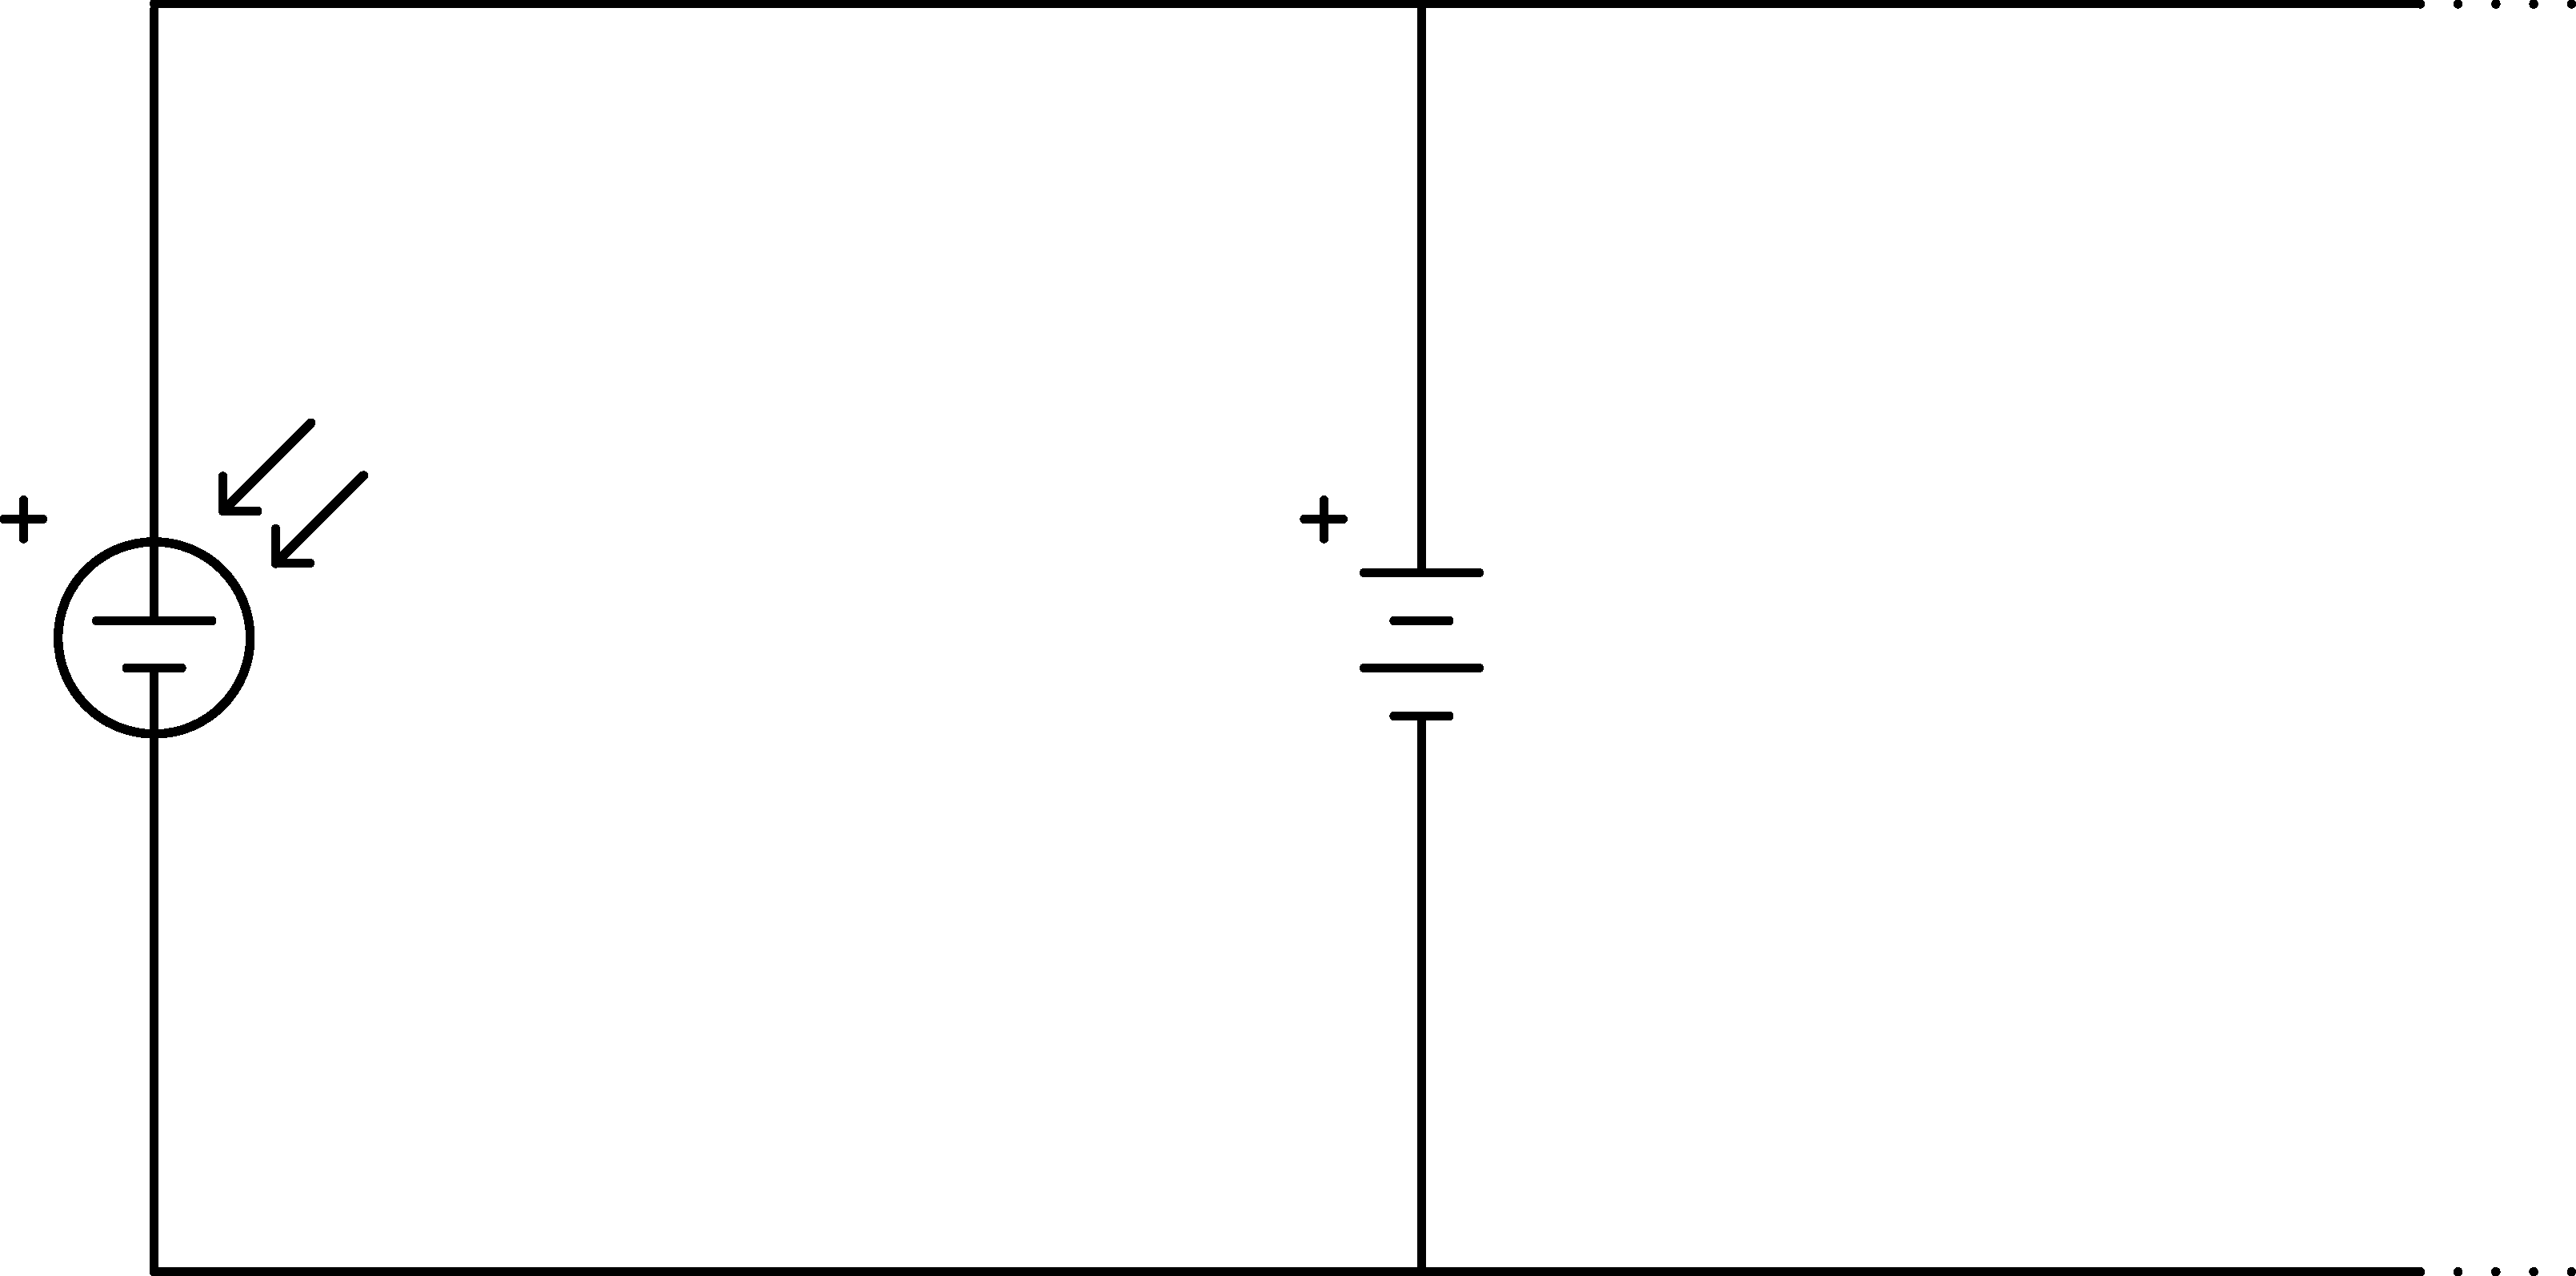
\includegraphics[width=0.75\linewidth]{versorgung_besipiel.pdf}
        \caption{Vereinfachte Darstellung der Stromversorgung}
    \end{figure}
    Dabei sind Steuer- und Regelelemente die das Speichermedium vor
    Schäden durch zu ofte Entladung schützen würden, sowie Filterelemente
    zur filterung Stromschwankungen ausgelassen.
    \newpage

    \section{Schlusswort}
    Bei ausreichend fester Regulation der Produktion zur Sicherhung
der Anwendung umweltfreundlicher Produktionverfahren kann Solar
in Verbindung mit anderen Erneuerbaren Energien als valide
Alternative zu fossilen Brennstoffen gesehen werden. Gerade zur
Zeit der Verfassung dieser Arbeit in der Bedenken an die Zukunft
unserer Umwelt immer größer werden lohnt es sich diese
Alternativen erneut zu betrachten. Ich hoffe in dieser Arbeit die
Vor- und Nachteil von Solarenergie sowie die Anwendungsgebiete
und Funktionsweise ausreichen beschrieben zu haben. Darüber
hinaus hoffe ich zum Nachdenken über erneuerbare Energien
angeregt zu haben.
    \newpage

    \newpage
\begin{thebibliography}{9}
    % Articles
    \bibitem{Wiki_SolarCell}
        \href{https://de.wikipedia.org/wiki/Solarzelle}{
            Wikipedia: Solarzelle
        }\\
        \href{https://en.wikipedia.org/wiki/Solar_cell}{
            Wikipedia: Solarcell (Englisch)
        }

    \bibitem{Wiki_PhotoelectricEffect}
        \href{https://de.wikipedia.org/wiki/Photoelektrischer_Effekt}{
            Wikipedia: Photoelektrischer Effekt
        }

    \bibitem{Wiki_PhotovoltaicHistory}
        \href{https://de.wikipedia.org/wiki/Geschichte_der_Photovoltaik}{
            Wikipedia: Geschichte der Photovoltaik
        }

    \bibitem{Wiki_Vanguard}
        \href{https://de.wikipedia.org/wiki/Vanguard-Projekt}{
            Wikipedia: Vanguard-Projekt
        }

    % Images
    \bibitem{Wiki_Img_PhotodiodeSymbol}
        \href{https://de.wikipedia.org/wiki/Datei:Symbol_Photodiode.svg}{
            Wikipedia: Symbol einer Photodiode
        }

    % Vidoes
    \bibitem{Wiki_Video_RE-SolarFlaw}
        \href{https://www.youtube.com/watch?v=yVOnHWnLSeU}{
            YouTube: Real Engineering - The Mystery Flaw of Solar Panels
        }

    \bibitem{Wiki_Video_RE-California}
        \href{https://www.youtube.com/watch?v=h5cm7HOAqZY}{
            YouTube: Real Engineering - California's Renewable Energy Problem
        }
\end{thebibliography}
\end{document}